\section{Controller design with exosystem in continuous time}
\label{system_design}

The main goal of the control is to make the system react faster to changes in the load. Along with the the inverter power, load changes affect the system as disturbances. The main task is then to reject these disturbances and make the closed-loop dynamics react faster to sudden changes coming from the load. This directly means that by applying a controller to the system, the error in voltage will be reduced on the output, and will go to zero as fast as it is possible. 
The dynamics of the system are changed through feeding back the states, thus the feedback law for the overall closed loop system becomes: 

\begin{equation}
  \label{eq:feedbacklaw}
  u = r + \mathbf{Fx}
  \end{equation}

It should be noted however, that due to the separation principle the state feedback and the observer problem can be handled independently and furthermore, while designing the state feedback for the system, disturbances can be neglected on the system. The block diagram of the system then simplifies to: 

%\begin{figure}[H]
%\centering
%\includegraphics[width=0.55\textwidth]{rapport/billeder/stateblock}
%\caption{State feedback}
%\label{fig:stateblock}
%\end{figure}

\begin{figure}[H]
\centering
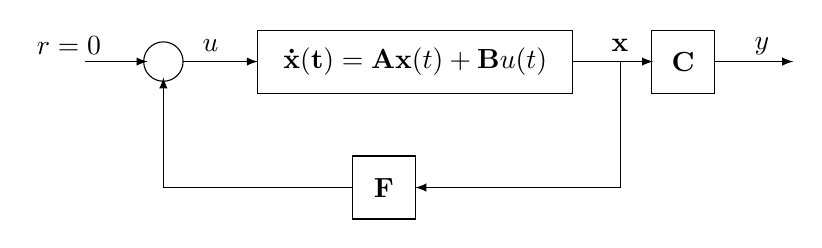
\begin{tikzpicture}

 \draw [-latex] (-0.4,2) ellipse (0.25 and 0.25);
\node at (2.8,2) {\normalsize{$\mathbf{\dot{x}(t)} = \mathbf{A} \mathbf{x}(t) + \mathbf{B} u(t) $}};

\draw [thin] (0.8,2.4) rectangle (4.8,1.6);
 \node at (6.2,2) {\normalsize{$\mathbf{C}$}};
\draw [thin] (5.8,2.4) rectangle (6.6,1.6);
 \node at (2.4,0.4) {\normalsize{$\mathbf{F}$}};


\draw [thin] (2,0.8) rectangle (2.8,0);
\draw [thin](4.67,2) node (v1) {};

\draw [-latex](v1) -- (5.82,2);
\draw [-latex](6.6,2) -- (7.6,2);
\draw [-latex](5.4,2) -- (5.4,0.4) -- (2.8,0.4);
\draw [-latex](-0.15,2) -- (0.8,2);
\draw [-latex](2,0.4) -- (-0.4,0.4) -- (-0.4,1.8);
\draw [-latex](-1.4,2) -- (-0.6,2);
\node at (0.2,2.2) {\normalsize{$u$}};
\node at (5.4,2.2) {\normalsize{$\mathbf{x}$}};
\node at (7.2,2.2) {\normalsize{$y$}};
\node at (-1.6,2.2) {\normalsize{$r = 0$}};
\end{tikzpicture}
\caption{State feedback}
\label{fig:statefeedback}
\end{figure}


Therefore the control problem simplifies to the problem of finding new locations of the eigenvalues such as:

\begin{equation}
  \label{eq:distpoly}
    det(s\mathbf{I}-(\mathbf{A} + \mathbf{B} \mathbf{F}))
  \end{equation}

Since these eigenvalues define the closed-loop dynamics, the main design decision is to find where to place them. The original poles of the system are: 
\begin{equation}
  \label{eq:original poles}
  p_{1;2} = -1.7 \pm j7
  \end{equation}

It can be clearly seen from \eqref{eq:original poles} that the system has a complex conjugate pole pair on the left-hand side of the real axis, therefore the system is stable, as it was expected. By placing the poles more than four times further, the following pole configuration can be achieved: 

\begin{equation}
  \label{eq:desired_poles}
  p_{F_{1;2}} = -8 \pm j7
  \end{equation}
  
The step response with state feedback yields: 
\begin{figure}[H]
\centering
\includegraphics[width=0.85\textwidth]{rapport/billeder/statefeedback}
\caption{State feedback.}
\label{fig:statefeedback}
\end{figure}


And the state feedback gain is the following:

\begin{equation}
\label{eq:ss_dist2}
    F
=
 \begin{bmatrix}
    -12.6 & -60.95
\end{bmatrix}
\end{equation}